\section{Modularização}
\label{sec:modulos}


\subsection{Lista de diretórios e arquivos}

{\small 
\begin{verbatim}
webscan
|-- ui
|   |-- index.html
|   |-- jquery-1.2.6.js
|   `-- scanner.js
`-- daemon
    |-- setup.py
    `-- webscan
        |-- __init__.py
        |-- lib
        |   |-- __init__.py
        |   |-- conf
        |   |   |-- __init__.py
        |   |   `-- global_settings.py
        |   |-- contrib
        |   |   |-- __init__.py
        |   |   |-- action
        |   |   |   |-- __init__.py
        |   |   |   |-- ocr.py
        |   |   |   `-- pdf.py
        |   |   `-- wrapper
        |   |       |-- Sane.py
        |   |       `-- __init__.py
        |   `-- core
        |       |-- __init__.py
        |       |-- action.py
        |       |-- driver_wrapper.py
        |       |-- scanners
        |       |   |-- __init__.py
        |       |   `-- scanners.py
        |       |-- type.py
        |       `-- user.py
        `-- server
            |-- __init__.py
            `-- django
                |-- __init__.py
                |-- example
                |   |-- __init__.py
                |   |-- manage.py
                |   |-- settings.py
                |   `-- urls.py
                |-- urls.py
                |-- utils.py
                `-- views
                    |-- __init__.py
                    |-- scanner.py
                    `-- user.py
\end{verbatim}}

\subsection{Módulo Daemon}
Este módulo é responsável pela interface com drivers dos scanners, 
execução de ações, escrita de arquivos em discos além de expor todos 
os métodos relevantes como webservices.

Todos os webservices utilizados retornam JSON e estão preparados para
serem executados através de chamadas 
cross-domain\footnote{http://en.wikipedia.org/wiki/Cross\_Domain\_Solutions}.

\subsubsection{Descrição de arquivos}

Os arquivos \_\_init\_\_.py são inicializadores de pacotes padrões na linguagem 
python e por este motivo não serão detalhados neste documento. Maiores detalhes
sobre o funcionamento de pacotes em python podem ser encontrados na documentação
oficial da 
linguagem\footnote{http://docs.python.org/tutorial/modules.html\#packages}.

\begin{itemize}
\item setup.py
\begin{verbatim}
Arquivo de instalação do projeto. Neste arquivo são definidos
os metadados utilizados para a geração de pacotes e instalação
do software. Este arquivo segue o padrão setuptools.
\end{verbatim}

\item webscan/
\begin{verbatim}
Diretório que contém todo o código-fonte do módulo daemon.
Este diretório é utilizado apenas para manter separação entre
os arquivos de instalação e dos arquivos fonte.  
\end{verbatim}

\item webscan/lib/
\begin{verbatim}
Contém tudo o que for utilizado por servidores para a execução
das tarefas de escaneamento e escrita em disco.
\end{verbatim}

\item webscan/lib/conf/
\begin{verbatim}
Contém o arquivo de configuração default.
\end{verbatim}

\item webscan/lib/conf/global\_settings.py
\begin{verbatim}
Arquivo de configuração default.
\end{verbatim}

\item webscan/lib/contrib/
\begin{verbatim}
Diretório que pode vir a receber arquivos externos
acopláveis ao sistema(como plugins).
\end{verbatim}

\item webscan/lib/contrib/action/
\begin{verbatim}
Contém as ações padrões que podem ser aplicadas em imagens 
sucessivamente.
\end{verbatim}

\item webscan/lib/contrib/action/ocr.py
\begin{verbatim}
Ação que extrai conteúdo textual das imagens.
\end{verbatim}

\item webscan/lib/contrib/action/pdf.py
\begin{verbatim}
Ação responsável pela geração de PDF's a partir de imagens. 
Pode ser utilizada em conjunto com a ação ocr para gerar 
documentos indexáveis.
\end{verbatim}

\item webscan/lib/contrib/wrapper/
\begin{verbatim}
Local onde ficam todos os wrappers para drivers e 
especificações de quando eles devem ser utilizados.
\end{verbatim}

\item webscan/lib/contrib/wrapper/Sane.py
\begin{verbatim}
Wrapper para os drivers sane. Utilizado em sistemas posix.
\end{verbatim}

\item webscan/lib/contrib/wrapper/Twain.py
\begin{verbatim}
Wrapper para os drivers Twain. Utilizado nas plataformas 
Windows.
\end{verbatim}

\item webscan/lib/core/
\begin{verbatim}
Núcleo do sistema responsável pelo processamento de ações, 
imagens, além de prover classes abstratas para criação de 
ações e wrappers.
\end{verbatim}

\item webscan/lib/core/action.py
\begin{verbatim}
Instruções responsáveis pelo processamento de ações.
\end{verbatim}

\item webscan/lib/core/driver\_wrapper.py
\begin{verbatim}
Classe abstrata para a construção de um wrapper.
\end{verbatim}

\item webscan/lib/core/type.py
\begin{verbatim}
Estruturas de dados utilizadas no projeto.
\end{verbatim}

\item webscan/lib/core/user.py
\begin{verbatim}
Rotinas criadas para tratar do espaço de usuário, incluindo
grupos de imagens e escrita em disco.
\end{verbatim}

\item webscan/lib/core/scanners/
\begin{verbatim}
Implementa o singleton coleção de scanners.
\end{verbatim}

\item webscan/lib/core/scanners/scanners.py
\begin{verbatim}
Funções utilizadas pela coleção de scanners.
\end{verbatim}

\item webscan/server/
\begin{verbatim}
Espaço reservado para implementação de métodos para a 
exposição da API, via HTTP.
\end{verbatim}

\item webscan/server/django/
\begin{verbatim}
Aplicação Django criada para expor os métodos do projeto
via HTTP.
\end{verbatim}

\item webscan/server/django/urls.py
\begin{verbatim}
Arquivo de mapeamento de URL's para funções (views).
\end{verbatim}

\item webscan/server/django/utils.py
\begin{verbatim}
Funções utilizadas por mais de uma view.
\end{verbatim}

\item webscan/server/django/example/
\begin{verbatim}
Instância exemplo da aplicação Django.
\end{verbatim}

\item webscan/server/django/example/manage.py
\begin{verbatim}
Arquivo criado, automaticamente, ao se criar um projeto 
Django.
\end{verbatim}

\item webscan/server/django/example/settings.py
\begin{verbatim}
Arquivo de configuração de um projeto Django.
\end{verbatim}

\item webscan/server/django/example/urls.py
\begin{verbatim}
Arquivo base de mapeamento de urls. Default em projetos 
Django.
\end{verbatim}

\item webscan/server/django/views/
\begin{verbatim}
Métodos wrappers utilizados para chamar funções do 
webscan.lib e modificar as saídas para formatos esperados
pelo Django.
\end{verbatim}

\item webscan/server/django/views/scanner.py
\begin{verbatim}
Implementa os wrappers necessários à implementação, dos 
métodos do objeto scanner utilizando Django.
\end{verbatim}

\item webscan/server/django/views/user.py
\begin{verbatim}
Implementa os wrappers das funções relacionadas diretamente
ao usuários do sistema.
\end{verbatim}

\end{itemize} 

\subsection{Módulo UI}
O módulo UI implementa a interface web utilizada para fazer chamadas assíncronas
ao módulo daemon. 

Este módulo é composto apenas por arquivos Javascript e HTML e utiliza a biblioteca Jquery
apresentada na seção \ref{sec:bibs}.

Segue abaixo algumas capturas de tela da interface desenvolvida.

\begin{figure}[ht]
\begin{center}
\scalebox{0.5} {
    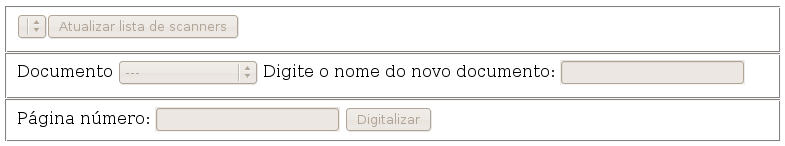
\includegraphics{imagens/lista_scanners.png}}
\end{center}
  \caption{Procura de scanners disponíveis}
  \label{fig:urls}
\end{figure}

\begin{figure}[ht]
\begin{center}
\scalebox{0.5} {
    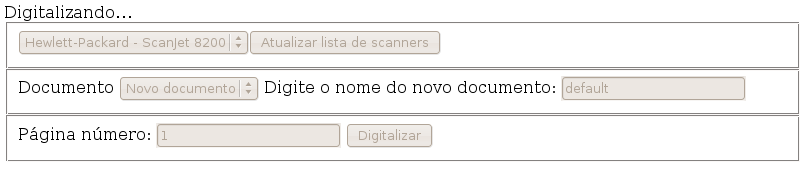
\includegraphics{imagens/digitalizando.png}}
\end{center}
  \caption{Digitalizando página em um novo documento}
  \label{fig:urls}
\end{figure}

\begin{figure}[ht]
\begin{center}
\scalebox{0.5} {
    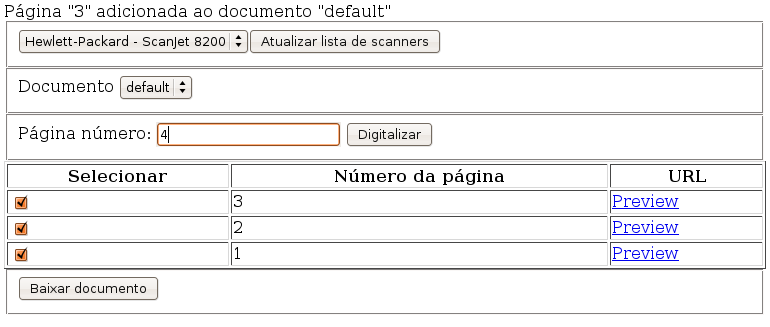
\includegraphics{imagens/digitalizado.png}}
\end{center}
  \caption{Mensagem de sucesso e lista de páginas digitalizadas}
  \label{fig:urls}
\end{figure}
